\documentclass[12pt]{book} 

\usepackage{amsmath}
\usepackage{graphicx}
\usepackage{import}
\usepackage{amsfonts}
\usepackage{booktabs}

\setlength{\parindent}{0em}  % sets auto indent at new paragraph to none

\newcommand{\incfig}[1]{%
    \import{./figures/}{#1.pdf_tex}
}

\title{\coursetitle\linebreak\lecturename}
\author{\\Cain Susko\\ 
           \\ \\ \\
      Queen's University 
    \\School of Computing\\} 

%=-=-=-=-=-title-=-=-=-=-=%
\newcommand{\lecturename}{Machine Representation, Fundamentals and Control}
\newcommand{\coursetitle}{Computer Architecture}
%=-=-=-=-=-#####-=-=-=-=-=%

\begin{document}
\begin{titlepage}
        \maketitle
\end{titlepage}


\section*{Complete Memory Addressing Modes}
\begin{itemize}
        \item[\texttt{D}] Constant Displacement
        \item[\texttt{Rb}] Base register: any of the 16 registers
        \item[\texttt{Ri}] Index register: any register except \texttt{\%rsp}
        \item[\texttt{S}] Scale: 1, 2, 4, 8 (only these numbers)
\end{itemize}

There are also some special cases:
\begin{figure}[h]
        \centering
        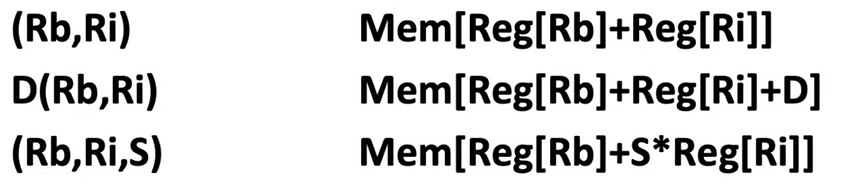
\includegraphics[scale = 0.5]{./figures/spclcase}
\end{figure}

Here are some examples of address computation.
\begin{figure}[h]
        \centering
        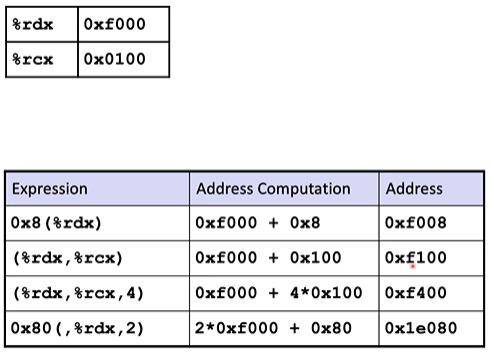
\includegraphics[scale = 0.7]{./figures/addressex}
\end{figure}
\pagebreak


\section*{Arithmetic and Logic Operations}
\paragraph{Address Computation Instruction}
Is denoted by \texttt{leaq\textit{ src }\textit{dest}}

Where \textit{src} is the address mode expression and sets \textit{dest} to address denoted by expression.

It can be used to compute memory addresses without a memory reference (In C this would be equiv. to \texttt{p = \&x[i]}

It can also be used for computing arithmetic expressions of the form $x + k*y$ where  $k = \{1,2,4,8\}$.
For example:
 \begin{figure}[h]
         \centering
         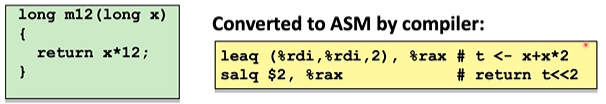
\includegraphics[scale = 0.7]{./figures/leaqex}
\end{figure}

There are also a host of other more common arithmetic operations:
\begin{figure}[h]
        \centering
        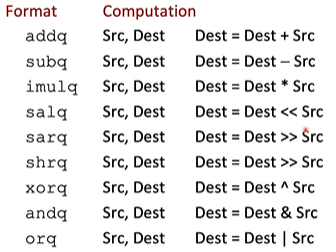
\includegraphics{./figures/arithops}
\end{figure}
Note that numbers are in 2's complement and \textbf{Watch Out} for the argument order. Also, there is no distinction between 
signed and unsigned integers.
\pagebreak


Here are some examples of Arithmetic operations with addresses:
\begin{figure}[h]
        \centering
        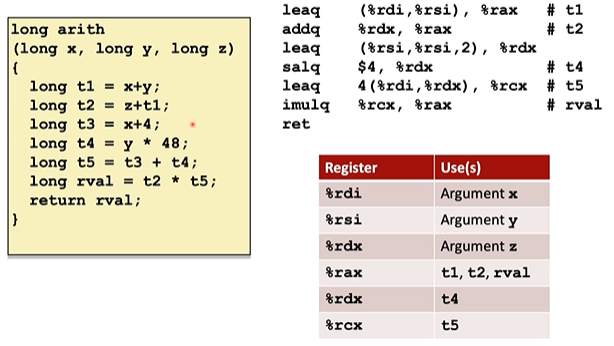
\includegraphics[scale = 0.7]{./figures/arithex}
\end{figure}

\section*{Summary - so far}
\begin{itemize}
        \item The History of Intel Processors / x86
        \item System assembly and machine code
        \item Assembly basics: registers, operands, etc.
        \item Arithmetic
\end{itemize}

\section*{Control}
Control aka Condition Codes are one of the four following:
\[
CF\;\;ZF\;\;SF\;\;OF
.\] 
\pagebreak


They are also known as status flags.
These control the flow of computation. They each do the following:
\begin{itemize}
        \item[$CF$] Carry Flag (for unsigned)
        \item[$SF$] Sign Flag (for signed)
        \item[$ZF$] Zero Flag
        \item[$OF$] Overflow Flag (for signed)
\end{itemize}

\subsection*{Implicitly Set Condition Codes}
Given the example $\texttt{addq src dest}\leftrightarrow \texttt{t = a+b}$ These flags are implicitly set in arithmetic operations:
\begin{itemize}
        \item $CF$ is set if there is an unsigned overflow (carry out most significant bit)
        \item $ZF$ is set if \texttt{t == 0} 
        \item $SF$ is set if  \texttt{t<0} (as signed)
        \item $OF$ is set if two's complement overflow (signed overflow)
\end{itemize}

Note: that these are not set by the \texttt{leaq} instruction

\subsection*{Explicitly Set Condition Codes}
We can set the flags explicitly by using \texttt{cmpq Src1 Src2}, which is like computing $a-b$ without setting a destination,
This will cause the following flags:
 \begin{figure}[h]
         \centering
         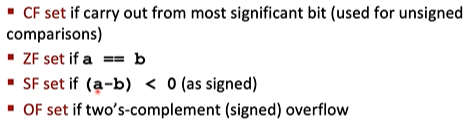
\includegraphics{./figures/explFlags}
 \end{figure}
\pagebreak


We can also explicitly set the flags by using the \texttt{testq Src1 Src2}, which is like computing $a\&\&b$ without setting a 
 destination.
 This will cause the following:
 \begin{figure}[h]
         \centering
         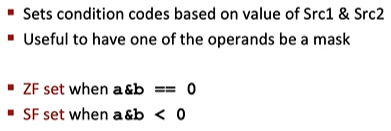
\includegraphics{./figures/explFlags2}
 \end{figure}

 \paragraph{Reading Condition Codes}
 We can use \texttt{SetX} instructions to set the low order byte destination to 1 or 0 based on the combinations of condition codes.
 They do note alter the remaining 7 bytes and are comprised of the following:
 \begin{figure}[h]
         \centering
         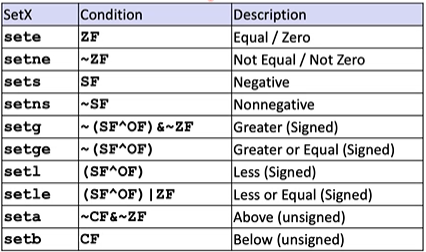
\includegraphics{./figures/setx}
 \end{figure}

 Note: typically use \texttt{movzbl} to finish the job.

 Below are some examples.
\pagebreak

\begin{figure}
        \centering
        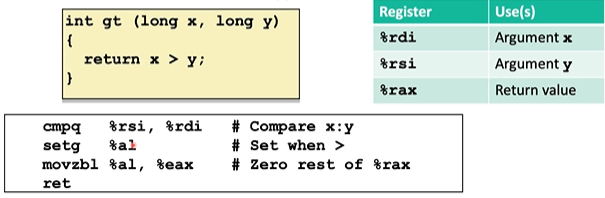
\includegraphics{./figures/readFlagEx}
\end{figure}

However, While this technique is useful, it is not how we will normally change flags. We will explore this in the next lesson


\end{document}

